% This is the Reed College LaTeX thesis template. Most of the work
% for the document class was done by Sam Noble (SN), as well as this
% template. Later comments etc. by Ben Salzberg (BTS). Additional
% restructuring and APA support by Jess Youngberg (JY).
% Your comments and suggestions are more than welcome; please email
% them to cus@reed.edu
%
% See http://web.reed.edu/cis/help/latex.html for help. There are a
% great bunch of help pages there, with notes on
% getting started, bibtex, etc. Go there and read it if you're not
% already familiar with LaTeX.
%
% Any line that starts with a percent symbol is a comment.
% They won't show up in the document, and are useful for notes
% to yourself and explaining commands.
% Commenting also removes a line from the document;
% very handy for troubleshooting problems. -BTS

% As far as I know, this follows the requirements laid out in
% the 2002-2003 Senior Handbook. Ask a librarian to check the
% document before binding. -SN

%%
%% Preamble
%%
% \documentclass{<something>} must begin each LaTeX document
\documentclass[12pt,twoside]{reedthesis}
% Packages are extensions to the basic LaTeX functions. Whatever you
% want to typeset, there is probably a package out there for it.
% Chemistry (chemtex), screenplays, you name it.
% Check out CTAN to see: http://www.ctan.org/
%%
\usepackage{graphicx,latexsym}
\usepackage{amsmath}
\usepackage{amssymb,amsthm}
\usepackage{longtable,booktabs,setspace}
\usepackage{chemarr} %% Useful for one reaction arrow, useless if you're not a chem major
\usepackage[hyphens]{url}
% Added by CII
\usepackage{hyperref}
\usepackage{lmodern}
\usepackage{float}
\floatplacement{figure}{H}
% End of CII addition
\usepackage{rotating}

% Next line commented out by CII
%%% \usepackage{natbib}
% Comment out the natbib line above and uncomment the following two lines to use the new
% biblatex-chicago style, for Chicago A. Also make some changes at the end where the
% bibliography is included.
%\usepackage{biblatex-chicago}
%\bibliography{thesis}


% Added by CII (Thanks, Hadley!)
% Use ref for internal links
\renewcommand{\hyperref}[2][???]{\autoref{#1}}
\def\chapterautorefname{Chapter}
\def\sectionautorefname{Section}
\def\subsectionautorefname{Subsection}
% End of CII addition

% Added by CII
\usepackage{caption}
\captionsetup{width=5in}
% End of CII addition

% \usepackage{times} % other fonts are available like times, bookman, charter, palatino

% Syntax highlighting #22
  \usepackage{color}
  \usepackage{fancyvrb}
  \newcommand{\VerbBar}{|}
  \newcommand{\VERB}{\Verb[commandchars=\\\{\}]}
  \DefineVerbatimEnvironment{Highlighting}{Verbatim}{commandchars=\\\{\}}
  % Add ',fontsize=\small' for more characters per line
  \usepackage{framed}
  \definecolor{shadecolor}{RGB}{248,248,248}
  \newenvironment{Shaded}{\begin{snugshade}}{\end{snugshade}}
  \newcommand{\AlertTok}[1]{\textcolor[rgb]{0.94,0.16,0.16}{#1}}
  \newcommand{\AnnotationTok}[1]{\textcolor[rgb]{0.56,0.35,0.01}{\textbf{\textit{#1}}}}
  \newcommand{\AttributeTok}[1]{\textcolor[rgb]{0.77,0.63,0.00}{#1}}
  \newcommand{\BaseNTok}[1]{\textcolor[rgb]{0.00,0.00,0.81}{#1}}
  \newcommand{\BuiltInTok}[1]{#1}
  \newcommand{\CharTok}[1]{\textcolor[rgb]{0.31,0.60,0.02}{#1}}
  \newcommand{\CommentTok}[1]{\textcolor[rgb]{0.56,0.35,0.01}{\textit{#1}}}
  \newcommand{\CommentVarTok}[1]{\textcolor[rgb]{0.56,0.35,0.01}{\textbf{\textit{#1}}}}
  \newcommand{\ConstantTok}[1]{\textcolor[rgb]{0.00,0.00,0.00}{#1}}
  \newcommand{\ControlFlowTok}[1]{\textcolor[rgb]{0.13,0.29,0.53}{\textbf{#1}}}
  \newcommand{\DataTypeTok}[1]{\textcolor[rgb]{0.13,0.29,0.53}{#1}}
  \newcommand{\DecValTok}[1]{\textcolor[rgb]{0.00,0.00,0.81}{#1}}
  \newcommand{\DocumentationTok}[1]{\textcolor[rgb]{0.56,0.35,0.01}{\textbf{\textit{#1}}}}
  \newcommand{\ErrorTok}[1]{\textcolor[rgb]{0.64,0.00,0.00}{\textbf{#1}}}
  \newcommand{\ExtensionTok}[1]{#1}
  \newcommand{\FloatTok}[1]{\textcolor[rgb]{0.00,0.00,0.81}{#1}}
  \newcommand{\FunctionTok}[1]{\textcolor[rgb]{0.00,0.00,0.00}{#1}}
  \newcommand{\ImportTok}[1]{#1}
  \newcommand{\InformationTok}[1]{\textcolor[rgb]{0.56,0.35,0.01}{\textbf{\textit{#1}}}}
  \newcommand{\KeywordTok}[1]{\textcolor[rgb]{0.13,0.29,0.53}{\textbf{#1}}}
  \newcommand{\NormalTok}[1]{#1}
  \newcommand{\OperatorTok}[1]{\textcolor[rgb]{0.81,0.36,0.00}{\textbf{#1}}}
  \newcommand{\OtherTok}[1]{\textcolor[rgb]{0.56,0.35,0.01}{#1}}
  \newcommand{\PreprocessorTok}[1]{\textcolor[rgb]{0.56,0.35,0.01}{\textit{#1}}}
  \newcommand{\RegionMarkerTok}[1]{#1}
  \newcommand{\SpecialCharTok}[1]{\textcolor[rgb]{0.00,0.00,0.00}{#1}}
  \newcommand{\SpecialStringTok}[1]{\textcolor[rgb]{0.31,0.60,0.02}{#1}}
  \newcommand{\StringTok}[1]{\textcolor[rgb]{0.31,0.60,0.02}{#1}}
  \newcommand{\VariableTok}[1]{\textcolor[rgb]{0.00,0.00,0.00}{#1}}
  \newcommand{\VerbatimStringTok}[1]{\textcolor[rgb]{0.31,0.60,0.02}{#1}}
  \newcommand{\WarningTok}[1]{\textcolor[rgb]{0.56,0.35,0.01}{\textbf{\textit{#1}}}}

% To pass between YAML and LaTeX the dollar signs are added by CII
\title{}
\author{}
% The month and year that you submit your FINAL draft TO THE LIBRARY (May or December)
\date{}
\division{}
\advisor{}
\institution{}
\degree{}
%If you have two advisors for some reason, you can use the following
% Uncommented out by CII
% End of CII addition

%%% Remember to use the correct department!
\department{}
% if you're writing a thesis in an interdisciplinary major,
% uncomment the line below and change the text as appropriate.
% check the Senior Handbook if unsure.
%\thedivisionof{The Established Interdisciplinary Committee for}
% if you want the approval page to say "Approved for the Committee",
% uncomment the next line
%\approvedforthe{Committee}

% Added by CII
%%% Copied from knitr
%% maxwidth is the original width if it's less than linewidth
%% otherwise use linewidth (to make sure the graphics do not exceed the margin)
\makeatletter
\def\maxwidth{ %
  \ifdim\Gin@nat@width>\linewidth
    \linewidth
  \else
    \Gin@nat@width
  \fi
}
\makeatother

\renewcommand{\contentsname}{Table of Contents}
% End of CII addition

\setlength{\parskip}{0pt}

% Added by CII

\providecommand{\tightlist}{%
  \setlength{\itemsep}{0pt}\setlength{\parskip}{0pt}}

\Acknowledgements{

}

\Dedication{

}

\Preface{

}

\Abstract{

}

% End of CII addition
%%
%% End Preamble
%%
%

\usepackage{amsthm}
\newtheorem{theorem}{Theorem}[chapter]
\newtheorem{lemma}{Lemma}[chapter]
\newtheorem{corollary}{Corollary}[chapter]
\newtheorem{proposition}{Proposition}[chapter]
\newtheorem{conjecture}{Conjecture}[chapter]
\theoremstyle{definition}
\newtheorem{definition}{Definition}[chapter]
\theoremstyle{definition}
\newtheorem{example}{Example}[chapter]
\theoremstyle{definition}
\newtheorem{exercise}{Exercise}[chapter]
\theoremstyle{remark}
\newtheorem*{remark}{Remark}
\newtheorem*{solution}{Solution}
\begin{document}

% Everything below added by CII

\frontmatter % this stuff will be roman-numbered
\pagestyle{empty} % this removes page numbers from the frontmatter



  \hypersetup{linkcolor=black}
  \setcounter{tocdepth}{2}
  \tableofcontents





\mainmatter % here the regular arabic numbering starts
\pagestyle{fancyplain} % turns page numbering back on

\hypertarget{abstract}{%
\section{Abstract}\label{abstract}}

\textbf{Context:} Large epidemiologic cohort studies, such as the
National Health and Nutrition Examination Survey (NHANES), collect
copious high-dimensional data that allow for examination of multiple
exposures in relation to a given outcome.

\textbf{Objective:} To explore the exposures measured in the Third
National Health and Nutrition Examination Survey (NHANES III) dataset in
search of factors associated with cancer mortality data obtained from
the National Death Index (NDI) and to assess methods for lethal cancer
risk prediction model variable selection.

\textbf{Methods:} We fit thousands of Cox proportional hazards models
with and without ridge penalties to randomly selected subsets of up to
50 variables. We analyzed the descriptions of NHANES variables provided
by NCHS and selected 3 variables that are important, non-modifiable risk
factors for cancer (age, sex and race/ethnicity) to include in all
future models. We then compared variables that appeared most frequently
in the Cox models with high significance (p \textless{}
10\textsuperscript{-10}) and selected 5 high-frequency, highly
significant variables that we used to train a new group of models with
fewer randomized variables.

\textbf{Results:} The models with selected variables outperformed the
fully randomized models in terms of concordance. Across all of the
models, the ten variables that most frequently surpassed the p-value
threshold were age, race/ethnicity, lifetime consumption of more than
100 cigarettes, 3 variables that pertain to physical activity and 3
variables that may be related to aging.

\textbf{Conclusions:} The work described here constitutes an exploratory
analysis of the NHANES III dataset that employs an iterative strategy
for the generation of cancer risk prediction models. Looking beyond this
demonstration of a variable selection method, our ultimate goal is to
build upon previously-described cancer risk factors towards the
discovery of novel contributors to cancer risk, a deeper understanding
of cancer etiology, and an improved ability to predict cancer incidence
and mortality.

\hypertarget{introduction}{%
\section{Introduction}\label{introduction}}

Cancer susceptibility is influenced by modifiable and non-modifiable
factors. Modifiable cancer risk factors include body mass index (BMI)
and cigarette use, whereas the non-modifiable factors include age, sex,
race/ethnicity, single nucleotide polymorphisms (SNPs), and family
history of disease. According to a 2018 study by Islami and colleagues
({\textbf{???}}), modifiable risk factors are responsible for 42\% of
all cancer cases and 45\% of all cancer deaths. This finding suggests
that cancer prevention strategies that target modifiable risk factors
have the potential to almost halve cancer incidence and mortality in the
United States. A near two-fold reduction in cancer cases and deaths may
seem far-fetched, but cancer incidence and mortality in United Status
have been declining by \textasciitilde{}1.5\% every year from 2009-2014
and 2001-2015, respectively ({\textbf{???}}). Taken together, these data
indicate that while tremendous progress has been made, there is still
great potential for cancer prevention approaches to decrease cancer
incidence and mortality.

The scale of cancer burden in the United States is staggering. Siegel
and colleagues estimate that in 2018 there will be 1.7 million newly
diagnosed cancer cases and roughly 600 thousand cancer deaths
({\textbf{???}}). Cancer risk prediction models can help policymakers
and cancer prevention practitioners develop more effective interventions
and to channel limited resources towards people at the greatest risk. To
achieve the best performance, cancer risk prediction models must include
both modifiable and non-modifiable risk factors. In 2016, Maas and
colleagues ({\textbf{???}}) demonstrated that cancer risk prediction
models based on known epidemiologic risk factors can be improved when
genetic information such as SNPs are included in the models.
Importantly, the combined model provided better risk stratification than
the models containing only epidemiologic risk factors or only genetic
variables.

The challenge of cancer risk prediction is complex and will require
cancer-type specific strategies that integrate multiple types of data
and explore various modeling methods. In addition to deepening our
understanding of known cancer risk factors, it is imperative to identify
new factors that may only be meaningful in the larger context of
contributors to cancer risk. This larger context includes the collection
of genetic inheritance, called the genome, and the myriad exposures that
individuals experience during their lives, known as the exposome
({\textbf{???}}).

Some genetic factors and environmental exposures may be very strongly
linked to cancer. Examples of well-described genetic and environmental
cancer risk factors include TP53 gene mutation in Li-Fraumeni Syndrome
and asbestos inhalation in mesothelioma, respectively. One of the
strongest cancer risk factors is cigarette smoking. In fact, smoking was
the strongest modifiable risk factor in the 2018 study by Islami and
colleagues ({\textbf{???}}). In this study, Islami and colleagues
determined that 19\% of all cancers cases and roughly 29\% of all
cancers deaths can be attributed to cigarette smoking ({\textbf{???}}).
To look beyond known cancer risk factors like cigarette smoking, new
cancer risk prediction models will need to detect small, but meaningful
effects amid a sea of other variables.

As part of the effort to tackle this challenge, we analyzed data from
\href{https://wwwn.cdc.gov/nchs/nhanes/nhanes3/DataFiles.aspx}{Third
National Health and Nutrition Examination Survey (NHANES III)}
({\textbf{???}}) and the accompanying
\href{https://www.cdc.gov/nchs/data-linkage/mortality-public.htm}{National
Death Index (NDI) Public-Use Linked Mortality Files}. The first goal of
the analysis was to explore the available NHANES III data and identify
potential variables of interest for cancer mortality risk prediction.
The second goal was to define an approach for variable selection for
cancer risk prediction models. NHANES III is different from many other
studies, in that instead of randomly sampling, NHANES utilizes a complex
design that employs probability-based sampling in multiple stages
({\textbf{???}}).

While the current work focuses solely on NHANES III, the data
exploration and variable selection methods described here can
potentially be applied to other studies, even those that have different
designs. For example, the Atherosclerosis Risk in Communities (ARIC)
study ({\textbf{???}}) and the Framingham Heart Study (FHS)
({\textbf{???}}) are, like NHANES, large cohort studies that do not
focus on cancer, but include relevant cancer outcomes as part of rich,
multidimensional datasets. In fact, the ARIC ({\textbf{???}}), NHANES
({\textbf{???}}), and FHS ({\textbf{???}}) datasets have already proven
useful for cancer research.

\hypertarget{methods}{%
\section{Methods}\label{methods}}

The Third National Health and Nutrition Examination Survey (NHANES III)
collected data on 33,994 participants aged 2 months and older from 1988
to 1994 in the United States. The data, which include Interview, Medical
Examination, and Laboratory components, were collected and linked with
Mortality data from NDI death certificate records by the National Center
for Health Statistics (NCHS) of the Centers for Disease Control and
Prevention (CDC). From the initial pool of participants, we selected
16404 adult (\(age \geq 18\)) participants who were cancer-free at
baseline and who had no missing values for follow-up time since
interview, NDI mortality, primary sampling units (PSU), stratification,
and sampling weight variables.

The initial publicly available dataset contained 3544 exposures from the
Interview, Medical Examination, Laboratory, and Mortality components.
After removing variables that were non-numeric, missing any values, only
had one unique value, or had correlation to another variable greater
than 0.9, we obtained the final set of 243 exposures. The analysis
described here did not involve multiple imputation nor utilize the
NHANES III Multiply Imputed Data Set. Among the 16404 participants,
there were 964 cancer deaths and 280891 total years of follow-up since
the initial Interview data were collected. The cancer deaths and
follow-up time were used as the outcome (survival) in Cox proportional
hazards regression analysis ({\textbf{???}}).

NHANES III data and documentation are available on the
\href{https://wwwn.cdc.gov/nchs/nhanes/nhanes3/DataFiles.aspx}{Centers
for Disease Control (CDC) - National Center for Health Statistics (NCHS)
website}. The National Death Index (NDI) linked mortality data are
available separately on the
\href{https://www.cdc.gov/nchs/data-linkage/mortality-public.htm}{Public-Use
Linked Mortality Files webpage}. We processed the Interview, Medical
Examination, and Laboratory, and Mortality data using the
\href{https://wwwn.cdc.gov/nchs/nhanes/nhanes3/DataFiles.aspx}{SAS code
provided by NCHS}, SAS University Edition version
\texttt{9.04.01M5P09132017} on a Jupyter Notebook ({\textbf{???}};
{\textbf{???}}) server version \texttt{5.1.0} running with Python
version \texttt{3.5.1} ({\textbf{???}}) on the Linux ({\textbf{???}})
operating system version \texttt{Red\ Hat\ 4.4.7-16} (with GNU Compiler
Collection version \texttt{4.4.7\ 20120313}).

We modified the SAS code to save the data as comma-separated-value
(\texttt{.csv}) files, which are available on
\href{https://figshare.com/articles/adult_csv/6210263}{FigShare}. The
SAS code files (\texttt{.sas}) and analogous Jupyter Notebook files
(\texttt{.ipynb}) are available on
\href{https://github.com/marskar/nhanes}{GitHub}. We then read the
\texttt{.csv} files into open-source R software ({\textbf{???}}) version
\texttt{3.5} using the \texttt{readr} R package ({\textbf{???}}). R has
a vibrant community and a rich ecosystem of software packages. All of
the software packages used in this work can be accessed from the
Comprehensive R Archive Network (CRAN) ({\textbf{???}}) or from GitHub
({\textbf{???}}) using the \texttt{devtools} package ({\textbf{???}}).

Next, we used the \texttt{dplyr} R package ({\textbf{???}}) to 1) remove
all NHANES participant identifiers (\texttt{SEQN}) without cause of
death (\texttt{UCOD\_LEADING}) or follow-up time from interview
(\texttt{PERMTH\_INT}) variables, 2) create a cancer mortality variable
based on whether the cause of death was ``Malignant neoplasms
(\texttt{C00-C97})'', and 3) join all four datasets together by the
participant identifier variable. From the combined dataset, we removed
baseline cancer cases (using the interview variables \texttt{HAC1N} and
\texttt{HAC1O}), participants that were missing the relevant NHANES
sampling variables (\texttt{SDDPSU6}, \texttt{SDSTRA6}, and
\texttt{WTPFQX6}), variables with a time origin other than the date of
interview (e.g. \texttt{PERMTH\_EXM} ), unnecessary NHANES sampling
variables, and variables that were based on or similar to the main age
variable (such as the age in months, \texttt{HSAITMOR}). To create the
final processed dataset, we also removed highly correlated variables
(\(r \geq 0.9\)) using the \texttt{caret} R package.

Methods to analyze complex survey data using SAS, SPSS, STATA, SUDAAN,
({\textbf{???}}) and R ({\textbf{???}}; {\textbf{???}}) software have
been described. From the final dataset, we randomly selected 1 to 50
predictor variables and trained Cox proportional hazards models with the
\texttt{survey} R package ({\textbf{???}}; {\textbf{???}}), which allows
for the analysis of complex survey design data using R ({\textbf{???}}).
In half of the models, we applied ridge penalties ({\textbf{???}}) to
the predictors variables using the \texttt{survival} R Package
({\textbf{???}}; {\textbf{???}}). In addition to the predictor
variables, the models also included 1) a ``survival object''
({\textbf{???}}; {\textbf{???}}) created from the event (cancer
mortality) and follow-up time variables and 2) a ``design object''
({\textbf{???}}) created from the Primary Sampling Unit
(\texttt{SDDPSU6}), Stratification (\texttt{SDSTRA6}) and Weight
(\texttt{WTPFQX6}) NHANES sampling variables\footnote{The
  \href{https://www.cdc.gov/nchs/tutorials/NHANES/SurveyDesign/SampleDesign/intro_iii.htm}{National
  Center for Health Statistics (NCHS)} recommends the application of the
  provided sampling design variables and sampling weights in all NHANES
  analyses.}.

We then calculated statistics describing the models and the variables
they contained and saved these statistics as \texttt{.rds} files using
the \texttt{readr} package ({\textbf{???}}). We automated the modeling
and statistical analyses using the \texttt{purrr} R package
({\textbf{???}}) and GNU Make ({\textbf{???}}). Specifically, the model
statistics collected were concordance ({\textbf{???}}) and Akaike
Information Criterion (AIC) ({\textbf{???}}) values, while the variable
statistics were p-values, hazard ratios, and hazard ratio confidence
intervals. We unpacked the model and variable data using the
\texttt{tidyr} R package ({\textbf{???}}).

Next, we selected 3 potential confounder variables representing age
(\texttt{HSAGEIR}) race/ethnicity (\texttt{DMAETHNR}), sex
(\texttt{HSSEX}) and repeated the modeling and statistical analysis
process described above. For the final modeling run, we chose an
additional 5 variables (\texttt{HAB1}, \texttt{HAR1}, \texttt{HAQ1},
\texttt{HAT2}, and \texttt{HAT10}) that appeared with high frequency as
highly significant (p-value \textless{} 10\textsuperscript{-10})
variables in the models we trained earlier. We joined all of the model
and variable statistics together, standardized column names using the
\texttt{stringr} ({\textbf{???}}) R package, and reordered the variable
names according to their counts using the \texttt{forcats}
({\textbf{???}}) R package. To make the final figures, the concordance
and AIC values (Figure 1), p-values and hazard ratios (Figure 2) and the
number of times each variable appeared in the models (Figure 3) were
plotted using the \texttt{ggplot2} R package ({\textbf{???}}).

\hypertarget{results}{%
\section{Results}\label{results}}

We present the data from thousands of Cox proportional hazards models (n
= 3789) we trained on NHANES III data in three iterative steps. The
Akaike Information Criterion (AIC) ({\textbf{???}}) and concordance
values ({\textbf{???}}) for all models are plotted in Figure 1. To
better understand the models created during the first iteration, we
divided the Group 1 models into 4 subgroups (1A, 1B, 1C, and 1D) based
on their AIC and concordance values. The models from the first iteration
(Figure 1; Groups 1A-D; green, cyan, blue, purple) were fully randomized
in terms of the predictor variables that were included, while the next
two iterations (Figure 1; Groups 2-3; orange, red) consisted of models
that started with 3 and 8 non-randomized variables, respectively, before
the addition of randomly chosen variables. The 3 variables included in
the second and third iteration were age, sex, and race/ethnicity,
whereas the final iteration contained an additional 5 variables, which
appeared frequently as highly significant (p \textless{}
10\textsuperscript{-10}) variables in the previous iterations. In all
cases, the models contained up to 50 predictor variables.

The models from the third iteration (Figure 1; Group 3; red) had the
highest concordance values overall, indicating that the addition of the
8 non-randomized predictor variables led to higher discriminatory power
between low and high-risk individuals. The gains in concordance seem to
be largely due to the addition of the age, sex, and race/ethnicity
variables as the concordance values we obtained from the second (Figure
1; Group 2; orange) and third (Figure 1; Group 3; red) iterations were
similar. Interestingly, models from the third iteration all had
concordance values of 84 or higher (Figure 1; black horizontal line),
while the range of AIC values was roughly the same in all three groups
of models (Figure 1). This finding suggests that while concordance can
differentiate between models from the three iterations, AIC by itself is
unable to make this distinction.
\begin{figure}
\centering
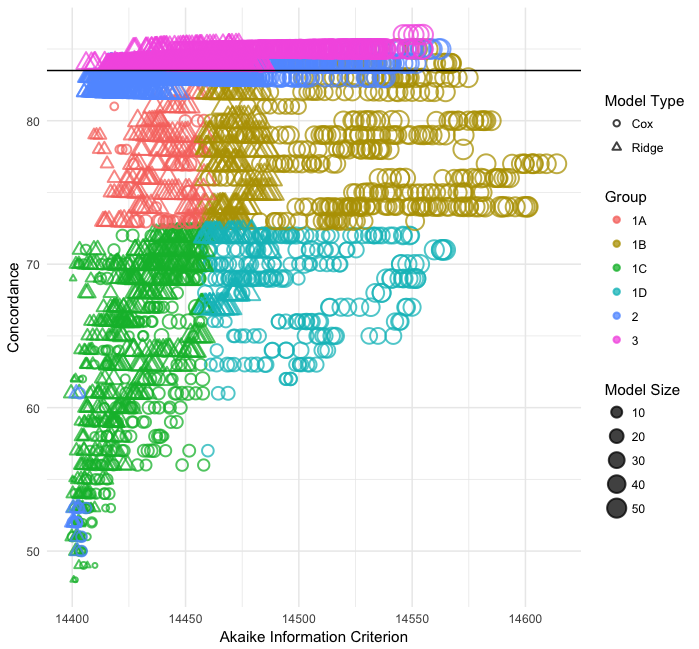
\includegraphics[width=1\textwidth,height=\textheight]{img/1-quad-final100dpi.png}
\caption{\textbf{Cancer Mortality Risk Prediction Models Trained on
NHANES III Data.} Each point in the scatter plot represents a Cox
proportional hazards model (n=3789) trained on NHANES III data. The
sizes of the points are relative to the number of variables (maximum =
50) in each the model, while the shapes correspond to whether ridge
penalties were applied (triangle) or not (circle). The colors of points
distinguish between models that had 0 (Groups 1A-D; green, cyan, blue,
purple), 3 (Group 2; orange) or 8 (Group 3; red) non-randomized
predictor variables. Additionally, Group 1 models are further color
coded by quadrants based on concordance and Akaike Information Criterion
(AIC) values as follows: high-concordance and low-AIC (Group 1A; green),
high-concordance and high-AIC (Group 1B; cyan), low-concordance and
low-AIC (Group 1C; blue), low-concordance and high-AIC (Group 1D;
purple). All Group 3 models have concordance values of 84 or higher
(black horizontal line).}
\end{figure}
The addition of a metric like AIC is important, because it serves to
provide a balance of goodness-of-fit and model complexity. Concordance,
unlike AIC, does not take into account the complexity of a model. As
follows, larger models tended to have higher concordance values, but
also higher AIC values. We applied ridge penalties ({\textbf{???}}),
also known as L2 regularization ({\textbf{???}}), to half of the models
from all three iterations, and noted that ridge penalization controls
this increase in AIC as models become larger (Figure 1). The
relationship between model size and concordance appears to plateau as
concordance increases (Figure 1), which suggests that the models are
reaching the limit of what is possible with the available 243 variables.
Though there is almost certainly another combination of variables that
would lead to further improvements in concordance, our approach allowed
us to generate a series of models that perform well without the need to
test every possible combination of the variables.

To choose variables to be included as non-randomized variables, we
consulted the NHANES variables descriptions available on the
\href{https://wwwn.cdc.gov/nchs/nhanes/nhanes3/DataFiles.aspx}{Centers
for Disease Control (CDC) - National Center for Health Statistics (NCHS)
website} and for the third iteration in particular we only considered
variables that had p-values lower than 10\textsuperscript{-10} (Figure
2; black horizontal line). It would be possible to introduce a threshold
for hazard ratios (Figure 2; x-axis), but this approach would tend to
select models without ridge penalties. The coefficients in ridge
penalized models are shrunk based on the penalty that is applied, which
in this case means that ridge penalized models have hazard ratios closer
to zero. While the significance and hazard ratios of variables depend on
the other variables in the model, our method allows us to survey the
landscape of p-values and hazard ratios of variables in the models
trained (Figure 2).
\begin{figure}
\centering
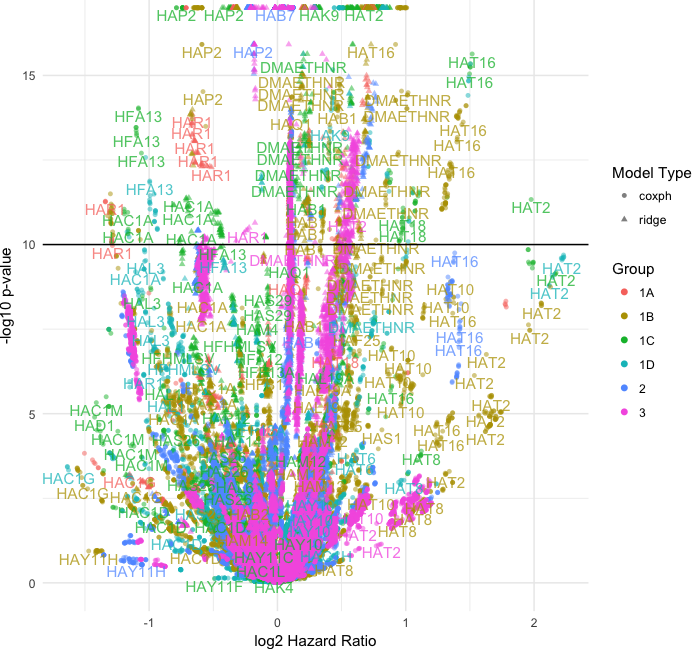
\includegraphics[width=1\textwidth,height=\textheight]{img/2-volcano-final100dpi.png}
\caption{\textbf{Predictor Variables from NHANES III Lethal Cancer Risk
Prediction Models.} Each point in the volcano plot represents a
predictor variable (n = 98787) from a Cox proportional hazards model (n
= 3789) trained on NHANES III data. Variables are considered to be
highly significant when their negative log10 p-values (y-axis) are above
10 (black horizontal line), regardless of their log2 hazard ratios
(x-axis). The shapes of points correspond to whether ridge penalties
were applied (triangle) or not (circle). The colors of points describe
the model each variable come from as in Figure 1.}
\end{figure}
The names, median hazard ratios, counts and descriptions of the ten most
frequent highly significant variables are summarized in Table 1. The
variable that appeared most frequently as highly significant across the
all of the models was age (Figure 3; \texttt{HSAGEIR}). When focusing on
the Group 1 models (Figure 3; Groups 1A-D; green, cyan, blue, purple),
the most frequent highly significant variable was an interview question
regarding dental health (Figure 3; \texttt{HAQ1}). The other top 10
high-frequency highly significant variables were race/ethnicity
(\texttt{DMAETHNR}), lifetime consumption of more than 100 cigarettes
(\texttt{HAR1}), 3 variables related to physical activity
(\texttt{HAT2}, \texttt{HAT10}, \texttt{HAT16}), and 3 variables that
may be associated to aging (\texttt{HAB7}, \texttt{HAK9}, and
\texttt{HAP2}). Interestingly, one of the variables, ``In the past 12
months, how many times were you in a nursing home?'' (\texttt{HAB7}),
was present as a highly significant variable only in the second and
third groups.
\begin{figure}
\centering
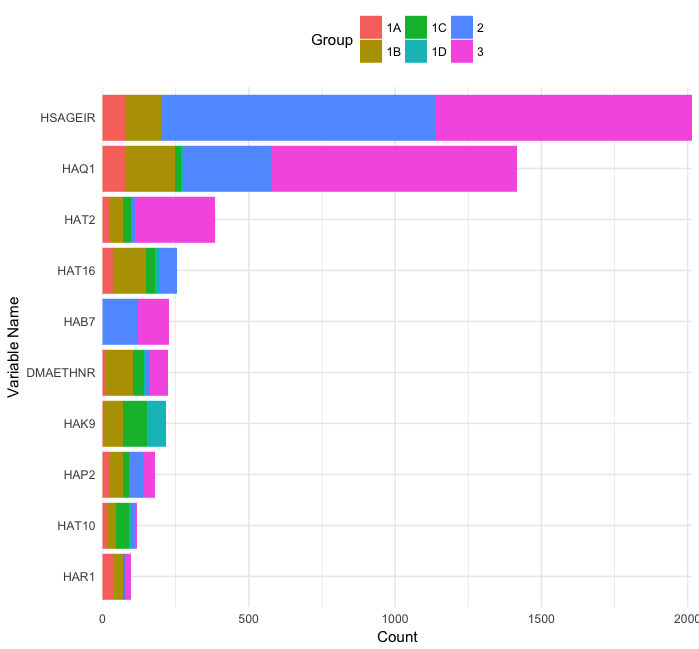
\includegraphics[width=1\textwidth,height=\textheight]{img/3-varbar-final100dpi.png}
\caption{The Ten Most Frequent, Highly Significant Predictor Variables.
Each row in the table represents one of the ten predictor variables that
appeared most frequently as highly significant (p \textless{}
10\textsuperscript{-10}) variables in the Cox models (n = 3789) trained
on NHANES III data. The median hazard ratio (HR) and count (n)
statistics are calculated on highly significant variables only. The
variables descriptions are based on the
\href{https://wwwn.cdc.gov/nchs/nhanes/nhanes3/DataFiles.aspx}{documentation
on the NHANES III website}.}
\end{figure}
\begin{longtable}[]{@{}lrrl@{}}
\caption{Description of Highly Significant Variables that Appeared Most
Frequently}\tabularnewline
\toprule
\begin{minipage}[b]{0.21\columnwidth}\raggedright
Name\strut
\end{minipage} & \begin{minipage}[b]{0.23\columnwidth}\raggedleft
Median HR\strut
\end{minipage} & \begin{minipage}[b]{0.12\columnwidth}\raggedleft
n\strut
\end{minipage} & \begin{minipage}[b]{0.33\columnwidth}\raggedright
Description\strut
\end{minipage}\tabularnewline
\midrule
\endfirsthead
\toprule
\begin{minipage}[b]{0.21\columnwidth}\raggedright
Name\strut
\end{minipage} & \begin{minipage}[b]{0.23\columnwidth}\raggedleft
Median HR\strut
\end{minipage} & \begin{minipage}[b]{0.12\columnwidth}\raggedleft
n\strut
\end{minipage} & \begin{minipage}[b]{0.33\columnwidth}\raggedright
Description\strut
\end{minipage}\tabularnewline
\midrule
\endhead
\begin{minipage}[t]{0.21\columnwidth}\raggedright
HSAGEIR\strut
\end{minipage} & \begin{minipage}[t]{0.23\columnwidth}\raggedleft
1.04\strut
\end{minipage} & \begin{minipage}[t]{0.12\columnwidth}\raggedleft
2016\strut
\end{minipage} & \begin{minipage}[t]{0.33\columnwidth}\raggedright
Age in Years\strut
\end{minipage}\tabularnewline
\begin{minipage}[t]{0.21\columnwidth}\raggedright
HAQ1\strut
\end{minipage} & \begin{minipage}[t]{0.23\columnwidth}\raggedleft
1.07\strut
\end{minipage} & \begin{minipage}[t]{0.12\columnwidth}\raggedleft
1415\strut
\end{minipage} & \begin{minipage}[t]{0.33\columnwidth}\raggedright
How would you describe the condition of your natural teeth (excellent,
very good, good, fair or poor)?\strut
\end{minipage}\tabularnewline
\begin{minipage}[t]{0.21\columnwidth}\raggedright
HAT2\strut
\end{minipage} & \begin{minipage}[t]{0.23\columnwidth}\raggedleft
1.50\strut
\end{minipage} & \begin{minipage}[t]{0.12\columnwidth}\raggedleft
384\strut
\end{minipage} & \begin{minipage}[t]{0.33\columnwidth}\raggedright
In the past month, did you jog or run?\strut
\end{minipage}\tabularnewline
\begin{minipage}[t]{0.21\columnwidth}\raggedright
HAT16\strut
\end{minipage} & \begin{minipage}[t]{0.23\columnwidth}\raggedleft
1.67\strut
\end{minipage} & \begin{minipage}[t]{0.12\columnwidth}\raggedleft
256\strut
\end{minipage} & \begin{minipage}[t]{0.33\columnwidth}\raggedright
In the past month, did you lift weights?\strut
\end{minipage}\tabularnewline
\begin{minipage}[t]{0.21\columnwidth}\raggedright
HAB7\strut
\end{minipage} & \begin{minipage}[t]{0.23\columnwidth}\raggedleft
0.99\strut
\end{minipage} & \begin{minipage}[t]{0.12\columnwidth}\raggedleft
228\strut
\end{minipage} & \begin{minipage}[t]{0.33\columnwidth}\raggedright
In the past 12 months, how many times were you in a nursing home?\strut
\end{minipage}\tabularnewline
\begin{minipage}[t]{0.21\columnwidth}\raggedright
DMAETHNR\strut
\end{minipage} & \begin{minipage}[t]{0.23\columnwidth}\raggedleft
1.14\strut
\end{minipage} & \begin{minipage}[t]{0.12\columnwidth}\raggedleft
224\strut
\end{minipage} & \begin{minipage}[t]{0.33\columnwidth}\raggedright
Race/Ethnicity\strut
\end{minipage}\tabularnewline
\begin{minipage}[t]{0.21\columnwidth}\raggedright
HAK9\strut
\end{minipage} & \begin{minipage}[t]{0.23\columnwidth}\raggedleft
1.23\strut
\end{minipage} & \begin{minipage}[t]{0.12\columnwidth}\raggedleft
216\strut
\end{minipage} & \begin{minipage}[t]{0.33\columnwidth}\raggedright
How many times per night do you usually get up to urinate?\strut
\end{minipage}\tabularnewline
\begin{minipage}[t]{0.21\columnwidth}\raggedright
HAP2\strut
\end{minipage} & \begin{minipage}[t]{0.23\columnwidth}\raggedleft
0.81\strut
\end{minipage} & \begin{minipage}[t]{0.12\columnwidth}\raggedleft
179\strut
\end{minipage} & \begin{minipage}[t]{0.33\columnwidth}\raggedright
Do you use glasses, contacts, or both?\strut
\end{minipage}\tabularnewline
\begin{minipage}[t]{0.21\columnwidth}\raggedright
HAT10\strut
\end{minipage} & \begin{minipage}[t]{0.23\columnwidth}\raggedleft
1.43\strut
\end{minipage} & \begin{minipage}[t]{0.12\columnwidth}\raggedleft
119\strut
\end{minipage} & \begin{minipage}[t]{0.33\columnwidth}\raggedright
In the past month, did you do other dancing?\strut
\end{minipage}\tabularnewline
\begin{minipage}[t]{0.21\columnwidth}\raggedright
HAR1\strut
\end{minipage} & \begin{minipage}[t]{0.23\columnwidth}\raggedleft
0.63\strut
\end{minipage} & \begin{minipage}[t]{0.12\columnwidth}\raggedleft
96\strut
\end{minipage} & \begin{minipage}[t]{0.33\columnwidth}\raggedright
Have you smoked at least 100 cigarettes during your entire life?\strut
\end{minipage}\tabularnewline
\bottomrule
\end{longtable}
The ranks of variables shown is Table 1 are determined by counts from
all 3789 models, and thus are heavily influenced by the fact that some
variables are included in all Group 2 (\texttt{HSAGEIR},
\texttt{DMAETHNR}, and \texttt{HSSEX}) and 3 models (\texttt{HSAGEIR},
\texttt{DMAETHNR}, \texttt{HSSEX}, \texttt{HAB1}, \texttt{HAR1},
\texttt{HAQ1}, \texttt{HAT2}, and \texttt{HAT10}). Table 1 therefore
serves as a summary of all three iterations of modeling and statistical
analysis. Rather than selecting the variables with the lowest p-values
or highest hazard ratios, we chose to follow a strategy that counts the
number of times a variable's significance crosses a p-value threshold.
This type of frequency-based ranking of variables can be used to both
guide future variable selection decisions and assess previous steps in
the model building process.

\hypertarget{discussion}{%
\section{Discussion}\label{discussion}}

To obtain a better understanding of how variables for cancer risk
prediction models can be selected, we utilized an iterative strategy to
explore the variables in the NHANES III dataset. As part of this
strategy, we randomly generated a large number of Cox proportional
hazards models to guide the training of new models with fewer randomly
chosen variables in future iterations. This method is akin to forward
subset selection ({\textbf{???}}) in that models are built up variable
by variable, but differs in that models are not assessed with the
addition of each new variable. In fact, the method we employed does not
take model performance metrics into consideration when selecting
variables. To inform variable selection in subsequent iterations, we
instead focused on the frequency with which variables had p-values below
10\textsuperscript{-10}.

The types of variables that were ranked highest in our present analysis
(age, race/ethnicity, smoking and physical activity) are all already
known to be strongly associated with cancer death. While obtaining the
expected result serves to confirm the validity of our method, the main
objective of this work is to provide insight that will lead to the
identification of new cancer risk factors. To this end, our method will
have to be refined to detect variables that weakly contribute to cancer
risk or whose contribution is context-specific. In essence, our current
approach aggregates information from across many models into a single
statistic per variable. Variable selection decisions could be informed
by another or a combination of other statistics.

For example, the significance threshold (p \textless{}
10\textsuperscript{-10}) we put in place was arbitrary and our method
could be used with a different threshold value, a different metric or a
combination of different thresholds. For example, variables could be
selected based on the number of times the absolute value of their hazard
ratio crosses a certain threshold. Model statistics could also be
employed for thresholds as the concordance, Akaike Information Criterion
(AIC) and other model performance metrics remain associated with
variables throughout all steps in the process.

In addition to changing the variable selection threshold, the method
described here could be adapted to use regularization techniques other
than ridge regression ({\textbf{???}}) and models other than Cox
proportional hazards models. In terms of regularization, survival
analyses can be done with lasso ({\textbf{???}}) penalties or a
combination of ridge and lasso penalties, which is known as Elastic Net
({\textbf{???}}). As for possible modeling algorithms to explore in the
future include tree-based models such as survival tree ({\textbf{???}}),
survival random forest models ({\textbf{???}}). Tree-based models are
easy to interpret and allow for the quantification of the proportion of
variance explained by variables included in the model. Another
statistical method called boosting, for example \texttt{XGBoost}
({\textbf{???}}), can be used to compute F-scores representing the
importance of each variable.

Regardless of the algorithms or thresholds used, the final result of our
approach is a new dataset of statistics that describe models and
variables across all iterations. This new dataset could be merged with
text data, such as the
\href{https://wwwn.cdc.gov/nchs/nhanes/nhanes3/DataFiles.aspx}{NHANES
III variable descriptions provided by the National Center for Health
Statistics}, and employ Natural Language Processing (NLP)
({\textbf{???}}) techniques to add further the information related to
the models and variables in the dataset. For example, NLP techniques
could be used to classify variables into categories, such as physical
activity or nutrition, based on their descriptions. All of this
information could then be combined with domain knowledge to steer the
variable selection process.

We demonstrated the ability of our method to generate models that
predict lethal cancer risk in the NHANES III dataset with high accuracy
(\(concordance \geq 84\)). It remains to be seen, whether our approach
could be generalizable to other studies and other outcomes. NHANES III
does not include cancer-type-specific mortality data, but other studies,
such as the Atherosclerosis Risk in Communities study (ARIC)
({\textbf{???}}; {\textbf{???}}), may provide the opportunity to
generate and assess models that predict mortality or incidence of a
specific type of cancer. As a continuation of this project, we expand
the methods described here into a general methodology that can be
applied beyond NHANES III to other large, high-dimensional cohort
studies. In addition to generalization to other studies, future work on
this project will include the creation of a software package that
encapsulates all of the relevant code and a graphical user interface
that facilitates data exploration, model parameter modification and
variable selection.

\hypertarget{connections-to-mph-goals-analysis}{%
\section{Connections to MPH Goals
Analysis}\label{connections-to-mph-goals-analysis}}

My MPH experience at Johns Hopkins has been absolutely transformative.
Though I started my MPH studies with a strong background in science, I
had no experience with public health or population science. Similarly,
while I was comfortable with R programming, I did not know the first
thing about survey data, let along how to conduct complex survey
analyses in R. In my Goals Analysis Plan, I outlined my goal of
broadening my horizons in three areas: substantive (domain) knowledge,
statistics (mathematics), and technical (programming) skills. , is This
NHANES III Research Report Capstone Project is testament to the skills I
honed and the knowledge I gained over the past year and also perfectly
aligns with my interests. I look forward to building upon this capstone
project as continue my career in cancer prevention research.

In terms of substantive knowledge, I wanted to focus on cancer
epidemiology

\hypertarget{references}{%
\section{References}\label{references}}

\hypertarget{rmd-basics}{%
\chapter{R Markdown Basics}\label{rmd-basics}}

Here is a brief introduction into using \emph{R Markdown}.
\emph{Markdown} is a simple formatting syntax for authoring HTML, PDF,
and MS Word documents. \emph{R Markdown} provides the flexibility of
\emph{Markdown} with the implementation of \textbf{R} input and output.
For more details on using \emph{R Markdown} see
\url{http://rmarkdown.rstudio.com}.

Be careful with your spacing in \emph{Markdown} documents. While
whitespace largely is ignored, it does at times give \emph{Markdown}
signals as to how to proceed. As a habit, try to keep everything left
aligned whenever possible, especially as you type a new paragraph. In
other words, there is no need to indent basic text in the Rmd document
(in fact, it might cause your text to do funny things if you do).

\hypertarget{lists}{%
\section{Lists}\label{lists}}

It's easy to create a list. It can be unordered like
\begin{itemize}
\tightlist
\item
  Item 1
\item
  Item 2
\end{itemize}
or it can be ordered like
\begin{enumerate}
\def\labelenumi{\arabic{enumi}.}
\tightlist
\item
  Item 1
\item
  Item 2
\end{enumerate}
Notice that I intentionally mislabeled Item 2 as number 4.
\emph{Markdown} automatically figures this out! You can put any numbers
in the list and it will create the list. Check it out below.

To create a sublist, just indent the values a bit (at least four spaces
or a tab). (Here's one case where indentation is key!)
\begin{enumerate}
\def\labelenumi{\arabic{enumi}.}
\tightlist
\item
  Item 1
\item
  Item 2
\item
  Item 3
  \begin{itemize}
  \tightlist
  \item
    Item 3a
  \item
    Item 3b
  \end{itemize}
\end{enumerate}
\hypertarget{line-breaks}{%
\section{Line breaks}\label{line-breaks}}

Make sure to add white space between lines if you'd like to start a new
paragraph. Look at what happens below in the outputted document if you
don't:

Here is the first sentence. Here is another sentence. Here is the last
sentence to end the paragraph. This should be a new paragraph.

\emph{Now for the correct way:}

Here is the first sentence. Here is another sentence. Here is the last
sentence to end the paragraph.

This should be a new paragraph.

\hypertarget{r-chunks}{%
\section{R chunks}\label{r-chunks}}

When you click the \textbf{Knit} button above a document will be
generated that includes both content as well as the output of any
embedded \textbf{R} code chunks within the document. You can embed an
\textbf{R} code chunk like this (\texttt{cars} is a built-in \textbf{R}
dataset):
\begin{verbatim}
     speed           dist       
 Min.   : 4.0   Min.   :  2.00  
 1st Qu.:12.0   1st Qu.: 26.00  
 Median :15.0   Median : 36.00  
 Mean   :15.4   Mean   : 42.98  
 3rd Qu.:19.0   3rd Qu.: 56.00  
 Max.   :25.0   Max.   :120.00  
\end{verbatim}
\hypertarget{inline-code}{%
\section{Inline code}\label{inline-code}}

If you'd like to put the results of your analysis directly into your
discussion, add inline code like this:
\begin{quote}
The \texttt{cos} of \(2 \pi\) is 1.
\end{quote}
Another example would be the direct calculation of the standard
deviation:
\begin{quote}
The standard deviation of \texttt{speed} in \texttt{cars} is 5.2876444.
\end{quote}
One last neat feature is the use of the \texttt{ifelse} conditional
statement which can be used to output text depending on the result of an
\textbf{R} calculation:
\begin{quote}
The standard deviation is less than 6.
\end{quote}
Note the use of \texttt{\textgreater{}} here, which signifies a
quotation environment that will be indented.

As you see with \texttt{\$2\ \textbackslash{}pi\$} above, mathematics
can be added by surrounding the mathematical text with dollar signs.
More examples of this are in \protect\hyperlink{math-sci}{Mathematics
and Science} if you uncomment the code in
\protect\hyperlink{math}{Math}.

\hypertarget{including-plots}{%
\section{Including plots}\label{including-plots}}

You can also embed plots. For example, here is a way to use the base
\textbf{R} graphics package to produce a plot using the built-in
\texttt{pressure} dataset:

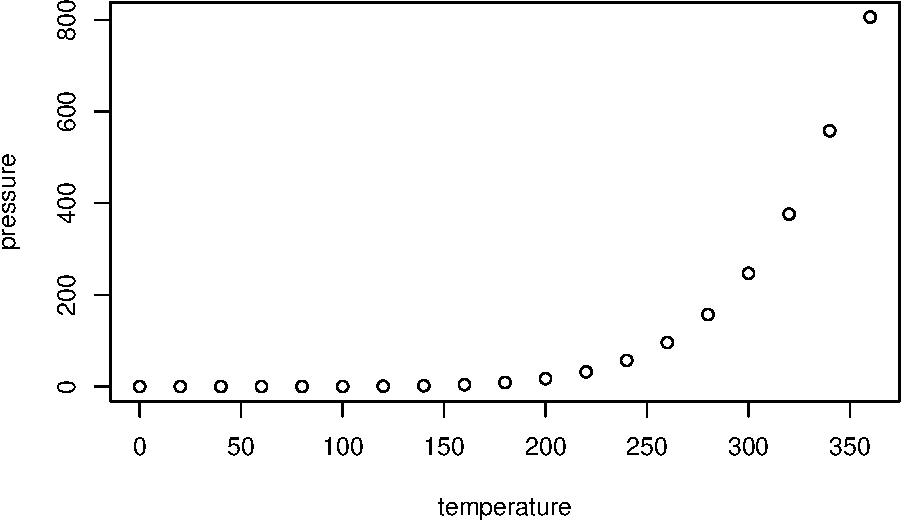
\includegraphics{thesis_files/figure-latex/pressure-1.pdf}

Note that the \texttt{echo=FALSE} parameter was added to the code chunk
to prevent printing of the \textbf{R} code that generated the plot.
There are plenty of other ways to add chunk options. More information is
available at \url{http://yihui.name/knitr/options/}.

Another useful chunk option is the setting of \texttt{cache=TRUE} as you
see here. If document rendering becomes time consuming due to long
computations or plots that are expensive to generate you can use knitr
caching to improve performance. Later in this file, you'll see a way to
reference plots created in \textbf{R} or external figures.

\hypertarget{loading-and-exploring-data}{%
\section{Loading and exploring data}\label{loading-and-exploring-data}}

Included in this template is a file called \texttt{flights.csv}. This
file includes a subset of the larger dataset of information about all
flights that departed from Seattle and Portland in 2014. More
information about this dataset and its \textbf{R} package is available
at \url{http://github.com/ismayc/pnwflights14}. This subset includes
only Portland flights and only rows that were complete with no missing
values. Merges were also done with the \texttt{airports} and
\texttt{airlines} data sets in the \texttt{pnwflights14} package to get
more descriptive airport and airline names.

We can load in this data set using the following command:

The data is now stored in the data frame called \texttt{flights} in
\textbf{R}. To get a better feel for the variables included in this
dataset we can use a variety of functions. Here we can see the
dimensions (rows by columns) and also the names of the columns.
\begin{verbatim}
[1] 52808    16
\end{verbatim}
\begin{verbatim}
 [1] "month"        "day"          "dep_time"     "dep_delay"   
 [5] "arr_time"     "arr_delay"    "carrier"      "tailnum"     
 [9] "flight"       "dest"         "air_time"     "distance"    
[13] "hour"         "minute"       "carrier_name" "dest_name"   
\end{verbatim}
Another good idea is to take a look at the dataset in table form. With
this dataset having more than 50,000 rows, we won't explicitly show the
results of the command here. I recommend you enter the command into the
Console \textbf{\emph{after}} you have run the \textbf{R} chunks above
to load the data into \textbf{R}.

While not required, it is highly recommended you use the \texttt{dplyr}
package to manipulate and summarize your data set as needed. It uses a
syntax that is easy to understand using chaining operations. Below I've
created a few examples of using \texttt{dplyr} to get information about
the Portland flights in 2014. You will also see the use of the
\texttt{ggplot2} package, which produces beautiful, high-quality
academic visuals.

We begin by checking to ensure that needed packages are installed and
then we load them into our current working environment:

\clearpage

The example we show here does the following:
\begin{itemize}
\item
  Selects only the \texttt{carrier\_name} and \texttt{arr\_delay} from
  the \texttt{flights} dataset and then assigns this subset to a new
  variable called \texttt{flights2}.
\item
  Using \texttt{flights2}, we determine the largest arrival delay for
  each of the carriers.
\end{itemize}
A useful function in the \texttt{knitr} package for making nice tables
in \emph{R Markdown} is called \texttt{kable}. It is much easier to use
than manually entering values into a table by copying and pasting values
into Excel or LaTeX. This again goes to show how nice reproducible
documents can be! (Note the use of \texttt{results="asis"}, which will
produce the table instead of the code to create the table.) The
\texttt{caption.short} argument is used to include a shorter title to
appear in the List of Tables.
\begin{longtable}[t]{lr}
\caption[Max Delays by Airline]{\label{tab:maxdelays}Maximum Delays by Airline}\\
\toprule
Airline & Max Arrival Delay\\
\midrule
Alaska Airlines Inc. & 338\\
American Airlines Inc. & 1539\\
Delta Air Lines Inc. & 651\\
Frontier Airlines Inc. & 575\\
Hawaiian Airlines Inc. & 407\\
\addlinespace
JetBlue Airways & 273\\
SkyWest Airlines Inc. & 421\\
Southwest Airlines Co. & 694\\
United Air Lines Inc. & 472\\
US Airways Inc. & 347\\
Virgin America & 366\\
\bottomrule
\end{longtable}
The last two options make the table a little easier-to-read.

We can further look into the properties of the largest value here for
American Airlines Inc.~To do so, we can isolate the row corresponding to
the arrival delay of 1539 minutes for American in our original
\texttt{flights} dataset.
\begin{verbatim}
  dep_time dep_delay arr_time tailnum flight dest air_time distance
1     1403      1553     1934  N595AA   1568  DFW      182     1616
\end{verbatim}
We see that the flight occurred on March 3rd and departed a little after
2 PM on its way to Dallas/Fort Worth. Lastly, we show how we can
visualize the arrival delay of all departing flights from Portland on
March 3rd against time of departure.

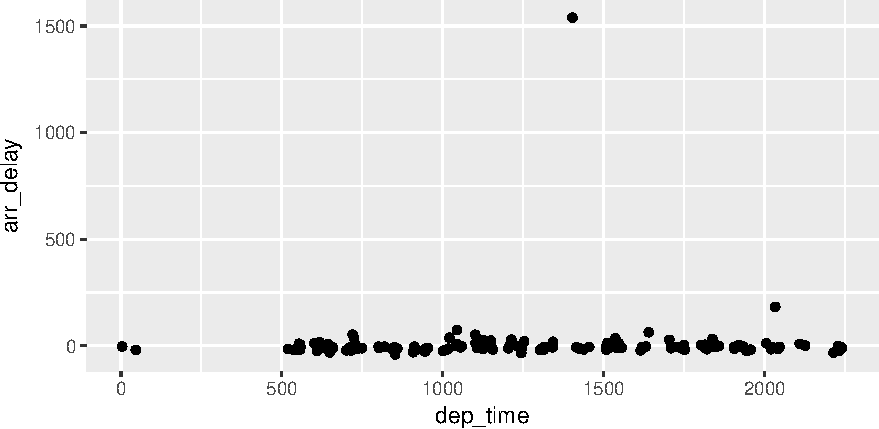
\includegraphics{thesis_files/figure-latex/march3plot-1.pdf}

\hypertarget{additional-resources}{%
\section{Additional resources}\label{additional-resources}}
\begin{itemize}
\item
  \emph{Markdown} Cheatsheet -
  \url{https://github.com/adam-p/markdown-here/wiki/Markdown-Cheatsheet}
\item
  \emph{R Markdown} Reference Guide -
  \url{https://www.rstudio.com/wp-content/uploads/2015/03/rmarkdown-reference.pdf}
\item
  Introduction to \texttt{dplyr} -
  \url{https://cran.rstudio.com/web/packages/dplyr/vignettes/introduction.html}
\item
  \texttt{ggplot2} Documentation -
  \url{http://docs.ggplot2.org/current/}
\end{itemize}
\hypertarget{math-sci}{%
\chapter{Mathematics and Science}\label{math-sci}}

\hypertarget{math}{%
\section{Math}\label{math}}

\TeX~is the best way to typeset mathematics. Donald Knuth designed
\TeX~when he got frustrated at how long it was taking the typesetters to
finish his book, which contained a lot of mathematics. One nice feature
of \emph{R Markdown} is its ability to read LaTeX code directly.

If you are doing a thesis that will involve lots of math, you will want
to read the following section which has been commented out. If you're
not going to use math, skip over or delete this next commented section.

\hypertarget{chemistry-101-symbols}{%
\section{Chemistry 101: Symbols}\label{chemistry-101-symbols}}

Chemical formulas will look best if they are not italicized. Get around
math mode's automatic italicizing in LaTeX by using the argument
\texttt{\$\textbackslash{}mathrm\{formula\ here\}\$}, with your formula
inside the curly brackets. (Notice the use of the backticks here which
enclose text that acts as code.)

So, \(\mathrm{Fe_2^{2+}Cr_2O_4}\) is written
\texttt{\$\textbackslash{}mathrm\{Fe\_2\^{}\{2+\}Cr\_2O\_4\}\$}.

\noindent Exponent or Superscript: \(\mathrm{O^-}\)

\noindent Subscript: \(\mathrm{CH_4}\)

To stack numbers or letters as in \(\mathrm{Fe_2^{2+}}\), the subscript
is defined first, and then the superscript is defined.

\noindent Bullet: CuCl \(\bullet\) \(\mathrm{7H_{2}O}\)

\noindent Delta: \(\Delta\)

\noindent Reaction Arrows: \(\longrightarrow\) or
\(\xrightarrow{solution}\)

\noindent Resonance Arrows: \(\leftrightarrow\)

\noindent Reversible Reaction Arrows: \(\rightleftharpoons\)

\hypertarget{typesetting-reactions}{%
\subsection{Typesetting reactions}\label{typesetting-reactions}}

You may wish to put your reaction in an equation environment, which
means that LaTeX will place the reaction where it fits and will number
the equations for you.
\begin{equation}
  \mathrm{C_6H_{12}O_6  + 6O_2} \longrightarrow \mathrm{6CO_2 + 6H_2O}
  \label{eq:reaction}
\end{equation}
We can reference this combustion of glucose reaction via Equation
\eqref{eq:reaction}.

\hypertarget{other-examples-of-reactions}{%
\subsection{Other examples of
reactions}\label{other-examples-of-reactions}}

\(\mathrm{NH_4Cl_{(s)}}\) \(\rightleftharpoons\)
\(\mathrm{NH_{3(g)}+HCl_{(g)}}\)

\noindent \(\mathrm{MeCH_2Br + Mg}\) \(\xrightarrow[below]{above}\)
\(\mathrm{MeCH_2\bullet Mg \bullet Br}\)

\hypertarget{physics}{%
\section{Physics}\label{physics}}

Many of the symbols you will need can be found on the math page
\url{http://web.reed.edu/cis/help/latex/math.html} and the Comprehensive
LaTeX Symbol Guide
(\url{http://mirror.utexas.edu/ctan/info/symbols/comprehensive/symbols-letter.pdf}).

\hypertarget{biology}{%
\section{Biology}\label{biology}}

You will probably find the resources at
\url{http://www.lecb.ncifcrf.gov/~toms/latex.html} helpful, particularly
the links to bsts for various journals. You may also be interested in
TeXShade for nucleotide typesetting
(\url{http://homepages.uni-tuebingen.de/beitz/txe.html}). Be sure to
read the proceeding chapter on graphics and tables.

\hypertarget{ref-labels}{%
\chapter{Tables, Graphics, References, and Labels}\label{ref-labels}}

\hypertarget{tables}{%
\section{Tables}\label{tables}}

In addition to the tables that can be automatically generated from a
data frame in \textbf{R} that you saw in
\protect\hyperlink{rmd-basics}{R Markdown Basics} using the
\texttt{kable} function, you can also create tables using \emph{pandoc}.
(More information is available at
\url{http://pandoc.org/README.html\#tables}.) This might be useful if
you don't have values specifically stored in \textbf{R}, but you'd like
to display them in table form. Below is an example. Pay careful
attention to the alignment in the table and hyphens to create the rows
and columns.
\begin{longtable}[]{@{}ccc@{}}
\caption{\label{tab:inher} Correlation of Inheritance Factors for Parents
and Child}\tabularnewline
\toprule
\begin{minipage}[b]{0.29\columnwidth}\centering
Factors\strut
\end{minipage} & \begin{minipage}[b]{0.47\columnwidth}\centering
Correlation between Parents \& Child\strut
\end{minipage} & \begin{minipage}[b]{0.16\columnwidth}\centering
Inherited\strut
\end{minipage}\tabularnewline
\midrule
\endfirsthead
\toprule
\begin{minipage}[b]{0.29\columnwidth}\centering
Factors\strut
\end{minipage} & \begin{minipage}[b]{0.47\columnwidth}\centering
Correlation between Parents \& Child\strut
\end{minipage} & \begin{minipage}[b]{0.16\columnwidth}\centering
Inherited\strut
\end{minipage}\tabularnewline
\midrule
\endhead
\begin{minipage}[t]{0.29\columnwidth}\centering
Education\strut
\end{minipage} & \begin{minipage}[t]{0.47\columnwidth}\centering
-0.49\strut
\end{minipage} & \begin{minipage}[t]{0.16\columnwidth}\centering
Yes\strut
\end{minipage}\tabularnewline
\begin{minipage}[t]{0.29\columnwidth}\centering
Socio-Economic Status\strut
\end{minipage} & \begin{minipage}[t]{0.47\columnwidth}\centering
0.28\strut
\end{minipage} & \begin{minipage}[t]{0.16\columnwidth}\centering
Slight\strut
\end{minipage}\tabularnewline
\begin{minipage}[t]{0.29\columnwidth}\centering
Income\strut
\end{minipage} & \begin{minipage}[t]{0.47\columnwidth}\centering
0.08\strut
\end{minipage} & \begin{minipage}[t]{0.16\columnwidth}\centering
No\strut
\end{minipage}\tabularnewline
\begin{minipage}[t]{0.29\columnwidth}\centering
Family Size\strut
\end{minipage} & \begin{minipage}[t]{0.47\columnwidth}\centering
0.18\strut
\end{minipage} & \begin{minipage}[t]{0.16\columnwidth}\centering
Slight\strut
\end{minipage}\tabularnewline
\begin{minipage}[t]{0.29\columnwidth}\centering
Occupational Prestige\strut
\end{minipage} & \begin{minipage}[t]{0.47\columnwidth}\centering
0.21\strut
\end{minipage} & \begin{minipage}[t]{0.16\columnwidth}\centering
Slight\strut
\end{minipage}\tabularnewline
\bottomrule
\end{longtable}
We can also create a link to the table by doing the following: Table
\ref{tab:inher}. If you go back to
\protect\hyperlink{loading-and-exploring-data}{Loading and exploring
data} and look at the \texttt{kable} table, we can create a reference to
this max delays table too: Table \ref{tab:maxdelays}. The addition of
the \texttt{(\textbackslash{}\#tab:inher)} option to the end of the
table caption allows us to then make a reference to Table
\texttt{\textbackslash{}@ref(tab:label)}. Note that this reference could
appear anywhere throughout the document after the table has appeared.

\clearpage

\hypertarget{figures}{%
\section{Figures}\label{figures}}

If your thesis has a lot of figures, \emph{R Markdown} might behave
better for you than that other word processor. One perk is that it will
automatically number the figures accordingly in each chapter. You'll
also be able to create a label for each figure, add a caption, and then
reference the figure in a way similar to what we saw with tables
earlier. If you label your figures, you can move the figures around and
\emph{R Markdown} will automatically adjust the numbering for you. No
need for you to remember! So that you don't have to get too far into
LaTeX to do this, a couple \textbf{R} functions have been created for
you to assist. You'll see their use below.

In the \textbf{R} chunk below, we will load in a picture stored as
\texttt{reed.jpg} in our main directory. We then give it the caption of
``Reed logo'', the label of ``reedlogo'', and specify that this is a
figure. Make note of the different \textbf{R} chunk options that are
given in the R Markdown file (not shown in the knitted document).
\begin{figure}
\centering

\includegraphics{figure/reed.jpg}
\caption{\label{fig:reedlogo}Reed logo}
\end{figure}
Here is a reference to the Reed logo: Figure \ref{fig:reedlogo}. Note
the use of the \texttt{fig:} code here. By naming the \textbf{R} chunk
that contains the figure, we can then reference that figure later as
done in the first sentence here. We can also specify the caption for the
figure via the R chunk option \texttt{fig.cap}.

\clearpage

Below we will investigate how to save the output of an \textbf{R} plot
and label it in a way similar to that done above. Recall the
\texttt{flights} dataset from Chapter \ref{rmd-basics}. (Note that we've
shown a different way to reference a section or chapter here.) We will
next explore a bar graph with the mean flight departure delays by
airline from Portland for 2014. Note also the use of the \texttt{scale}
parameter which is discussed on the next page.
\begin{figure}
\centering
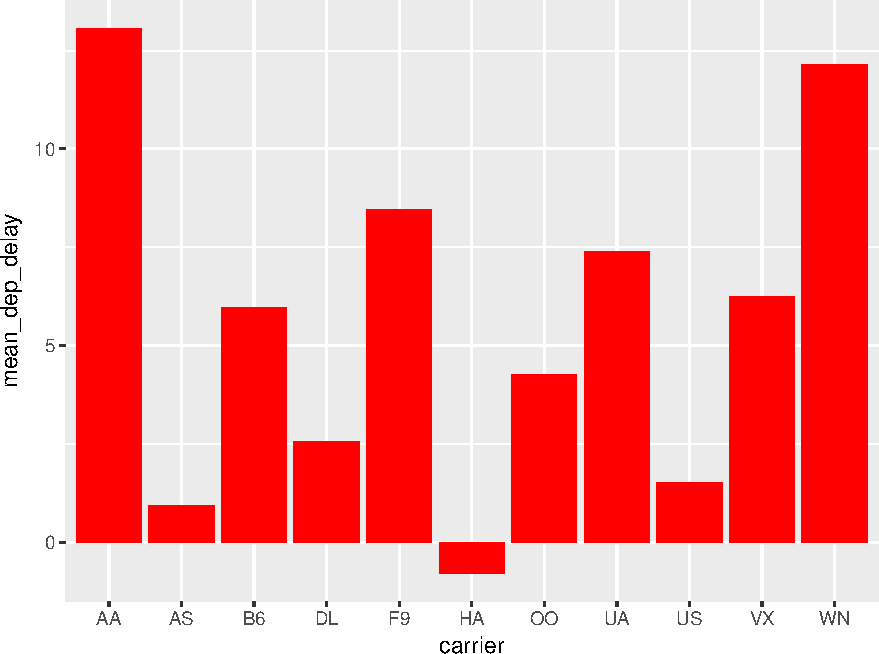
\includegraphics{thesis_files/figure-latex/delaysboxplot-1.pdf}
\caption{\label{fig:delaysboxplot}Mean Delays by Airline}
\end{figure}
Here is a reference to this image: Figure \ref{fig:delaysboxplot}.

A table linking these carrier codes to airline names is available at
\url{https://github.com/ismayc/pnwflights14/blob/master/data/airlines.csv}.

\clearpage

Next, we will explore the use of the \texttt{out.extra} chunk option,
which can be used to shrink or expand an image loaded from a file by
specifying \texttt{"scale=\ "}. Here we use the mathematical graph
stored in the ``subdivision.pdf'' file.
\begin{figure}
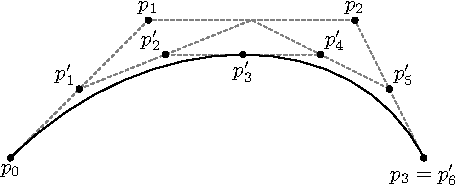
\includegraphics[scale=0.75]{figure/subdivision} \caption{Subdiv. graph}\label{fig:subd}
\end{figure}
Here is a reference to this image: Figure \ref{fig:subd}. Note that
\texttt{echo=FALSE} is specified so that the \textbf{R} code is hidden
in the document.

\textbf{More Figure Stuff}

Lastly, we will explore how to rotate and enlarge figures using the
\texttt{out.extra} chunk option. (Currently this only works in the PDF
version of the book.)
\begin{figure}
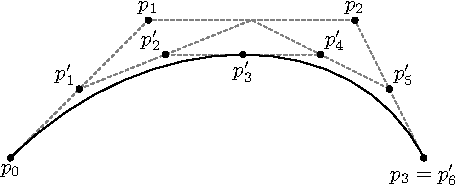
\includegraphics[angle=180, scale=1.1]{figure/subdivision} \caption{A Larger Figure, Flipped Upside Down}\label{fig:subd2}
\end{figure}
As another example, here is a reference: Figure \ref{fig:subd2}.

\hypertarget{footnotes-and-endnotes}{%
\section{Footnotes and Endnotes}\label{footnotes-and-endnotes}}

You might want to footnote something.\footnote{footnote text} The
footnote will be in a smaller font and placed appropriately. Endnotes
work in much the same way. More information can be found about both on
the CUS site or feel free to reach out to
\href{mailto:data@reed.edu}{\nolinkurl{data@reed.edu}}.

\hypertarget{bibliographies}{%
\section{Bibliographies}\label{bibliographies}}

Of course you will need to cite things, and you will probably accumulate
an armful of sources. There are a variety of tools available for
creating a bibliography database (stored with the .bib extension). In
addition to BibTeX suggested below, you may want to consider using the
free and easy-to-use tool called Zotero. The Reed librarians have
created Zotero documentation at
\url{http://libguides.reed.edu/citation/zotero}. In addition, a tutorial
is available from Middlebury College at
\url{http://sites.middlebury.edu/zoteromiddlebury/}.

\emph{R Markdown} uses \emph{pandoc} (\url{http://pandoc.org/}) to build
its bibliographies. One nice caveat of this is that you won't have to do
a second compile to load in references as standard LaTeX requires. To
cite references in your thesis (after creating your bibliography
database), place the reference name inside square brackets and precede
it by the ``at'' symbol. For example, here's a reference to a book about
worrying: ({\textbf{???}}). This \texttt{Molina1994} entry appears in a
file called \texttt{thesis.bib} in the \texttt{bib} folder. This
bibliography database file was created by a program called BibTeX. You
can call this file something else if you like (look at the YAML header
in the main .Rmd file) and, by default, is to placed in the \texttt{bib}
folder.

For more information about BibTeX and bibliographies, see our CUS site
(\url{http://web.reed.edu/cis/help/latex/index.html})\footnote{({\textbf{???}})}.
There are three pages on this topic: \emph{bibtex} (which talks about
using BibTeX, at \url{http://web.reed.edu/cis/help/latex/bibtex.html}),
\emph{bibtexstyles} (about how to find and use the bibliography style
that best suits your needs, at
\url{http://web.reed.edu/cis/help/latex/bibtexstyles.html}) and
\emph{bibman} (which covers how to make and maintain a bibliography by
hand, without BibTeX, at
\url{http://web.reed.edu/cis/help/latex/bibman.html}). The last page
will not be useful unless you have only a few sources.

If you look at the YAML header at the top of the main .Rmd file you can
see that we can specify the style of the bibliography by referencing the
appropriate csl file. You can download a variety of different style
files at \url{https://www.zotero.org/styles}. Make sure to download the
file into the csl folder.

\textbf{Tips for Bibliographies}
\begin{itemize}
\tightlist
\item
  Like with thesis formatting, the sooner you start compiling your
  bibliography for something as large as thesis, the better. Typing in
  source after source is mind-numbing enough; do you really want to do
  it for hours on end in late April? Think of it as procrastination.
\item
  The cite key (a citation's label) needs to be unique from the other
  entries.
\item
  When you have more than one author or editor, you need to separate
  each author's name by the word ``and'' e.g.
  \texttt{Author\ =\ \{Noble,\ Sam\ and\ Youngberg,\ Jessica\},}.
\item
  Bibliographies made using BibTeX (whether manually or using a manager)
  accept LaTeX markup, so you can italicize and add symbols as
  necessary.
\item
  To force capitalization in an article title or where all lowercase is
  generally used, bracket the capital letter in curly braces.
\item
  You can add a Reed Thesis citation\footnote{({\textbf{???}})} option.
  The best way to do this is to use the phdthesis type of citation, and
  use the optional ``type'' field to enter ``Reed thesis'' or
  ``Undergraduate thesis.''
\end{itemize}
\hypertarget{anything-else}{%
\section{Anything else?}\label{anything-else}}

If you'd like to see examples of other things in this template, please
contact the Data @ Reed team (email
\href{mailto:data@reed.edu}{\nolinkurl{data@reed.edu}}) with your
suggestions. We love to see people using \emph{R Markdown} for their
theses, and are happy to help.

\hypertarget{conclusion}{%
\chapter*{Conclusion}\label{conclusion}}
\addcontentsline{toc}{chapter}{Conclusion}

If we don't want Conclusion to have a chapter number next to it, we can
add the \texttt{\{-\}} attribute.

\textbf{More info}

And here's some other random info: the first paragraph after a chapter
title or section head \emph{shouldn't be} indented, because indents are
to tell the reader that you're starting a new paragraph. Since that's
obvious after a chapter or section title, proper typesetting doesn't add
an indent there.

\appendix

\hypertarget{the-first-appendix}{%
\chapter{The First Appendix}\label{the-first-appendix}}

This first appendix includes all of the R chunks of code that were
hidden throughout the document (using the \texttt{include\ =\ FALSE}
chunk tag) to help with readibility and/or setup.

\textbf{In the main Rmd file}
\begin{Shaded}
\begin{Highlighting}[]
\CommentTok{# This chunk ensures that the thesisdown package is}
\CommentTok{# installed and loaded. This thesisdown package includes}
\CommentTok{# the template files for the thesis.}
\ControlFlowTok{if}\NormalTok{(}\OperatorTok{!}\KeywordTok{require}\NormalTok{(devtools))}
  \KeywordTok{install.packages}\NormalTok{(}\StringTok{"devtools"}\NormalTok{, }\DataTypeTok{repos =} \StringTok{"http://cran.rstudio.com"}\NormalTok{)}
\ControlFlowTok{if}\NormalTok{(}\OperatorTok{!}\KeywordTok{require}\NormalTok{(thesisdown))}
\NormalTok{  devtools}\OperatorTok{::}\KeywordTok{install_github}\NormalTok{(}\StringTok{"ismayc/thesisdown"}\NormalTok{)}
\KeywordTok{library}\NormalTok{(thesisdown)}
\end{Highlighting}
\end{Shaded}
\textbf{In Chapter \ref{ref-labels}:}
\begin{Shaded}
\begin{Highlighting}[]
\CommentTok{# This chunk ensures that the thesisdown package is}
\CommentTok{# installed and loaded. This thesisdown package includes}
\CommentTok{# the template files for the thesis and also two functions}
\CommentTok{# used for labeling and referencing}
\ControlFlowTok{if}\NormalTok{(}\OperatorTok{!}\KeywordTok{require}\NormalTok{(devtools))}
  \KeywordTok{install.packages}\NormalTok{(}\StringTok{"devtools"}\NormalTok{, }\DataTypeTok{repos =} \StringTok{"http://cran.rstudio.com"}\NormalTok{)}
\ControlFlowTok{if}\NormalTok{(}\OperatorTok{!}\KeywordTok{require}\NormalTok{(dplyr))}
    \KeywordTok{install.packages}\NormalTok{(}\StringTok{"dplyr"}\NormalTok{, }\DataTypeTok{repos =} \StringTok{"http://cran.rstudio.com"}\NormalTok{)}
\ControlFlowTok{if}\NormalTok{(}\OperatorTok{!}\KeywordTok{require}\NormalTok{(ggplot2))}
    \KeywordTok{install.packages}\NormalTok{(}\StringTok{"ggplot2"}\NormalTok{, }\DataTypeTok{repos =} \StringTok{"http://cran.rstudio.com"}\NormalTok{)}
\ControlFlowTok{if}\NormalTok{(}\OperatorTok{!}\KeywordTok{require}\NormalTok{(ggplot2))}
    \KeywordTok{install.packages}\NormalTok{(}\StringTok{"bookdown"}\NormalTok{, }\DataTypeTok{repos =} \StringTok{"http://cran.rstudio.com"}\NormalTok{)}
\ControlFlowTok{if}\NormalTok{(}\OperatorTok{!}\KeywordTok{require}\NormalTok{(thesisdown))\{}
  \KeywordTok{library}\NormalTok{(devtools)}
\NormalTok{  devtools}\OperatorTok{::}\KeywordTok{install_github}\NormalTok{(}\StringTok{"ismayc/thesisdown"}\NormalTok{)}
\NormalTok{  \}}
\KeywordTok{library}\NormalTok{(thesisdown)}
\NormalTok{flights <-}\StringTok{ }\KeywordTok{read.csv}\NormalTok{(}\StringTok{"data/flights.csv"}\NormalTok{)}
\end{Highlighting}
\end{Shaded}
\hypertarget{the-second-appendix-for-fun}{%
\chapter{The Second Appendix, for
Fun}\label{the-second-appendix-for-fun}}

\backmatter

\hypertarget{references-1}{%
\chapter*{References}\label{references-1}}
\addcontentsline{toc}{chapter}{References}

\markboth{References}{References}

\noindent

\setlength{\parindent}{-0.20in}
\setlength{\leftskip}{0.20in}
\setlength{\parskip}{8pt}


% Index?

\end{document}
